\documentclass[xcolor=table]{beamer}
\usepackage{amsmath,amssymb,amsfonts,latexsym}

%\usepackage{icml2013} 
%\usepackage[latin1]{inputenc}
\usepackage{pgfgantt}
\usepackage[spanish]{babel}
\usepackage[utf8]{inputenc}
\usepackage[T1]{fontenc}
\usepackage{listings}
\usepackage{colortbl}
\usepackage[table]{xcolor}

% For algorithms
\usepackage{algorithm}
\usepackage{algorithmic}
% Incluir figuras .pdf, .png, .jpg, .gif, .eps, etc. SIN extensi\’on
%\usepackage{epstopdf}
%\DeclareGraphicsExtensions{.pdf,.png,.jpg,.gif, .eps}
\usefonttheme{professionalfonts} % fuentes de LaTeX
\usetheme{Warsaw}
% tema escogido en este ejemplo
\setbeamercovered{transparent}
% Velos
\newtheorem{Teorema}{Teorema}
\newtheorem{Ejemplo}{Ejemplo}
\newtheorem{Definicion}{Definición}
\newtheorem{Corolario}{Corolario}
\newtheorem{Prueba}{Prueba}
\begin{document}


\title{Mapa Caótico Renyi y su aplicación a algoritmos de cifrado de datos.\\}

\author{   {\bf        Marcos Daniel C. Calderón}      \\ 
{Seminario de Avance de Tesis  -  CIMAT}\\ 
{Asesor: Dr. Rogelio Hasimoto Beltrán}\\
\vspace*{0.5cm}}
\date{31 de enero de 2014}
\frame{\titlepage}

\section{Objetivo de la Tesis.}

\begin{frame}
\frametitle{Objetivo.}
La finalidad de este trabajo es encontrar nuevos métodos de cifrado de datos por medio de mapas caóticos acoplados. Se buscan nuevas alternativas que ofrezcan una mayor resistencia a ataques y donde se aprovechen los beneficios de los sistemas caóticos. Los resultados obtenidos se aplicarán al cifrado de imágenes. 
\end{frame}


\section{Conceptos Básicos.}

\begin{frame}
\frametitle{Sistema de cifrado.}

\begin{block}{Definición.}
Un sistema criptográfico es una quíntupla ($\mathbf{P}$ , $\mathbf{C}$ ,  $\mathbf{K}$ , $\mathbf{E}$ , $\mathbf{D}$), donde se satisfacen las siguientes condiciones:
\begin{itemize}
\item $\mathbf{P} $ es un conjunto finito de símbolos que forman un texto ''original''.
\item $\mathbf{C} $ es un conjunto finito de símbolos que forman un texto cifrado.
\item $\mathbf{K} $ es un conjunto finito de posibles claves.
\item Por cada $k \in \mathbf{K}$ existen funciones $e_{k} \in \mathbf{E}$  y $ d_{k} \in \mathbf{D}$, donde  cada $e_{k}: \mathbf{P} \rightarrow \mathbf{C}$ y $ d_{K}:  \mathbf{C} \rightarrow \mathbf{P}$ son funciones  que cumplen $d_{K}(e_{K}(x))=x$ para cada elemento del texto original $x \in \mathbf{P}$.
\end{itemize}
\end{block}
\end{frame}


\begin{frame}
\frametitle{Esquema de cifrado.}
\begin{figure}[H]
\centering
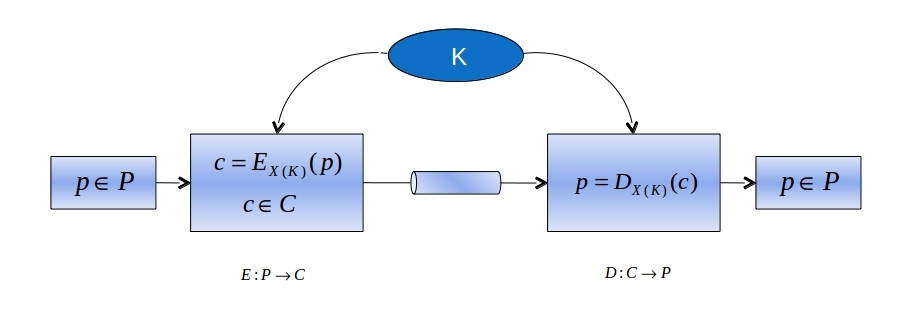
\includegraphics[width=10cm]{kakaka.jpg}
\end{figure}
\end{frame}


\begin{frame}{Números aleatorios y pseudoaleatorios.}

\begin{block}{Definición.}
Un \textit{\textbf{generador aleatorio de bits}} es un dispositivo o algoritmo que produce una secuencia de dígitos binarios estadísticamente independientes y uniformemente distribuidos.
\end{block}

\begin{block}{Definición.}
Un \textit{\textbf{generador pseudoaleatorio de bits}} es un algoritmo determinístico que, dada una secuencia binaria verdaderamente aleatoria; normalmente conocida como ''semilla'', genera múltiples bits pseudoaletorios que ''parecen'' ser al azar. Estos algoritmos se utilizan en la generación de claves.
\end{block}
\end{frame}


\begin{frame}
\frametitle{Sistema dinámico caótico.}
\begin{block}{Definición.}
Un \textbf{\textit{sistema dinámico caótico}} se caracteriza por tener un comportamiento en el tiempo complejo e impredecible. Normalmente, estos sistemas están representados por un grupo de ecuaciones diferenciales o discretas.
\end{block}


\end{frame}



\begin{frame}
\frametitle{Sistema dinámico caótico.}
\framesubtitle{Características.}

\small
\begin{table}[h]
\centering
\begin{tabular}{|l|p{5cm} |}
\hline
\cellcolor{blue!25}Propiedad caótica &\cellcolor{blue!25}Propiedad Criptográfica \\   \hline
Ergodicidad. & Confusión. \\ \hline
Sensibilidad a las condiciones iniciales. & Hay difusión con un pequeño cambio en el texto plano o llave secreta.  \\ \hline
Propiedad de mezclado. & Hay difusión con un pequeño cambio en un bloque del texto plano, o un cambio en la totalidad del mismo.\\ \hline
Dinámica determinística. & Pseudoaleatoriedad determinística. \\ \hline
Estructura compleja. & Complejidad para atacar un algoritmo.\\ \hline
\end{tabular} 
\end{table}
\end{frame}



\begin{frame}
\frametitle{Generador Caótico de Números Pseudoaleatorios Renyi...}

Consideremos el mapa caótico Renyi $\phi_{\beta}(x): [0,1)\longrightarrow [0,1)$ definido como:
\begin{equation}
\phi_{\beta}(x)= (\beta \cdot x) \mod 1
\end{equation}

Además, la siguiente expresión nos devolverá números en el intervalo $[0,1)$:
\begin{equation}
\hat{x} \in \mathbf{Q}: \hat{x}= \frac{k}{2^{n}}, \quad k \in \mathbf{N}, \quad k< 2^{n}
\end{equation}
\end{frame}



\begin{frame}
\frametitle{Generador Caótico de Números Pseudoaleatorios Renyi...}

Una aproximaxión de truncamiento es considerada para la evaluación de $\hat{x}$ en $\phi_{\beta}(x)$:

\begin{equation}
 \hat{\phi} _{\beta}(\hat{x})= (\beta \cdot  \hat{x})_{tr} \mod 1 = \lfloor (2^{n} \cdot \beta \cdot \hat{x}) \mod 2^{n}  \rfloor \cdot 2^{-n}
\end{equation}

Por medio del isomorfismo $k = \hat{x}\cdot 2^{n}$, el espacio definido en la ecuación (2) puede ser relacionado con un conjunto de números naturales:

\begin{equation}
\Lambda _{n}= { k \in \mathbf{N} }, \quad 0 \leq k < 2^{n}
\end{equation}
\end{frame}

\begin{frame}
\frametitle{Generador Caótico de Números Pseudoaleatorios Renyi...}

Podemos definir una función $f: \Lambda_{n} \longrightarrow  \Lambda_{n} $ así:

\begin{equation}
f(k)= 2^{n}  \hat{\phi} _{\beta}(2^{-n}k)=  \lfloor \beta \cdot k \mod 2^{n}  \rfloor =
\lfloor  \beta \cdot k \rfloor \mod 2^{n}
\end{equation}


El parámetro $\beta$ puede ser escrito como la suma de una parte entera $b$ y una fracción $\gamma$, por lo tanto, (5) puede ser escrito así:

\begin{equation}
f(k)= (bk + \lfloor \gamma \cdot k \rfloor) \mod 2^{n}
\end{equation}
\end{frame}


\begin{frame}
\frametitle{Generador Caótico de Números Pseudoaleatorios Renyi.}

La parte fraccional de la ecuación (6) puede ser escrita como: $\gamma = 2^{-j}$ para algún entero $j>0$. Por lo tanto, obtenemos la expresión final del mapa caótico Renyi:

\begin{equation}
f(k)=  \left( q 2^{n-i}k+  \lfloor\frac{k}{2^{j}} \rfloor   \right) \mod 2^{n}.
\end{equation}
\end{frame}





\begin{frame}
\frametitle{Sistemas caóticos acoplados.}
\begin{block}{Acoplamiento.}
Este fenómeno ocurre cuando dos sistemas dinámicos interactúan entre sí. Por ejemplo:
\begin{equation}
C' =  \alpha C - \beta CZ
\end{equation}

\begin{equation}
Z' = - \gamma Z + \delta CZ
\end{equation}
Se dice que el sistema es acoplado porque las razones de cambio de C y Z dependen tanto de C como de Z. 
\end{block}


\end{frame}



\begin{frame}
\frametitle{Ejemplo: Redes de Mapas.}
\begin{equation}
X_{i,j}=(1 - \epsilon)f(X_{i,j-1})+ \epsilon H(X_{1,j-1},...,X_{N,j-1})
\end{equation}
\begin{itemize}
\item La interacción entre diferentes mapas provoca en un sistema caótico, ciclos de mayor tamaño: H representa una transformación de acoplamiento.

\item  Aparece el fenómeno de sincronización, que consiste en un régimen en el cual los sistemas caóticos acoplados, después de un tiempo de transición, exhiben oscilaciones caóticas idénticas.
\end{itemize}

\end{frame}




\begin{frame}
\frametitle{Pruebas de aleatoriedad.}
\begin{itemize}
\item En una prueba de aleatoriedad, se establece como falsa a priori, una Hipótesis nula: ''Los símbolos analizados son independientes entre sí y uniformemente distribuídos''. Lo que se busca es evaluar el grado de aleatoriedad de la secuencia para validar la Hipótesis nula.
\item \textbf{NIST} es un paquete de 16 exámenes estadísticos, se han desarrollado para probar la aleatoriedad de una secuencia de bits producida por un generador de números pseudoaleatorio o aleatorio.
\end{itemize}
\end{frame}


\section{Resultados.}



\begin{frame}
\frametitle{Pruebas NIST mapa Renyi.}
\framesubtitle{Resultados obtenidos.}

\begin{table}[!h]
\label{sample-table}

\begin{center}
\begin{small}
\begin{sc}
\scalebox{0.8}{
\begin{tabular}{lccr}
\hline
Prueba Aplicada &  P-Valor & Exito? \\
\hline

Aproximate Entropy    &  0.303647   & $\surd$ \\

Block Frecuency  &  0.450408  &  $\surd$  \\

Cumulative Sums    &   Forward test: 0.777054, Reverse test: 0.671857   & $\surd$ \\

FFT    &   0.617327 &   $\surd$      \\

Frecuency     &  0.820988  &  $\surd$   \\

Linear Complexity      & 0.784292 & $\surd$ \\

Longest Run      &  0.795471 &    $\surd$      \\

Non Overlapping Template      & P-valores aceptados: 148 de 148    &     $\surd$          \\

Overlapping Template      & 0.642080 &        $\surd$       \\

Random Excursions      & P-valores aceptados: 8 de 8  &     $\surd$          \\

Random Excursions Variant & P-valores aceptados: 18 de 18  &    $\surd$        \\

Rank &    0.707380      &       $\surd$      \\

Runs &        0.265730    &     $\surd$        \\

Serial &     P-valores aceptados: 2 de 2     &     $\surd$        \\

Universal &     0.696176  &   $\surd$            \\
\hline
\end{tabular}}
\end{sc}
\end{small}
\end{center}
\end{table}
\end{frame}


\begin{frame}
\frametitle{Comportamiento.}
\begin{figure}[H]
\centering
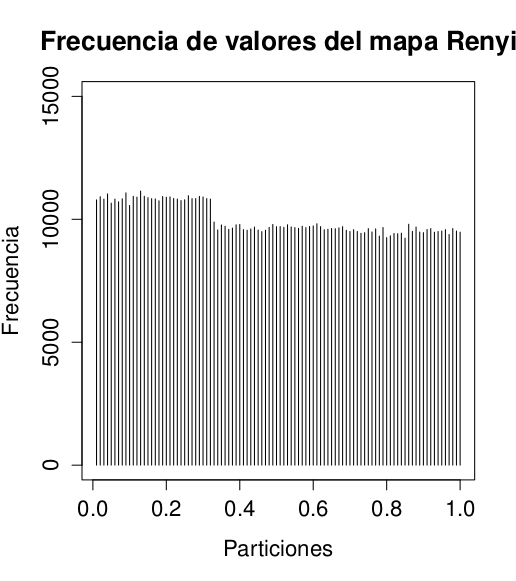
\includegraphics[width=6cm]{pit.jpg}
\end{figure}
\end{frame}




\begin{frame}
\frametitle{Tamaños de ciclo.}
También es importante obtener secuencias de números pseudoaleatorios donde el tamaño de un ciclo sea muy grande.
\begin{figure}[H]
\centering
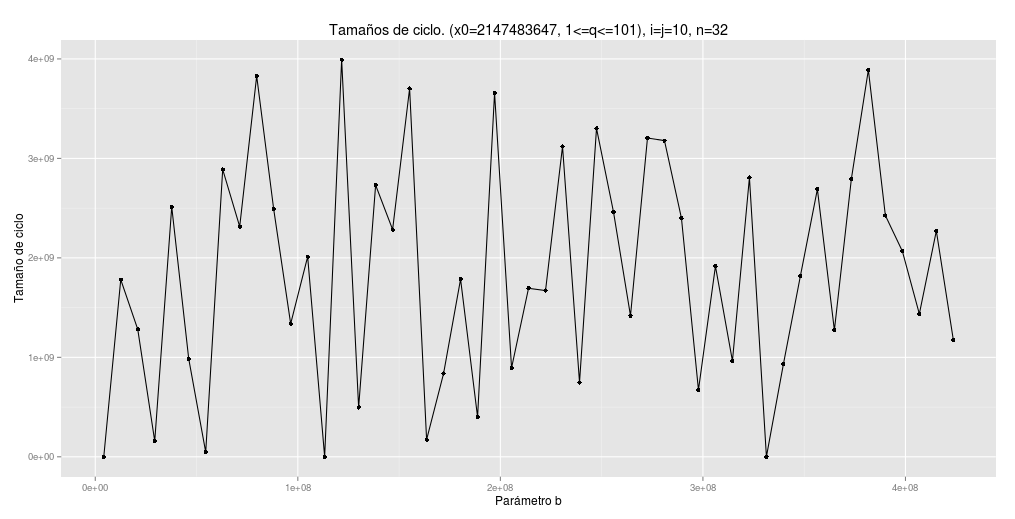
\includegraphics[width=10cm]{jaja.png}
%\caption{Tamaños de ciclo.}\label{figtam}
\end{figure}
\end{frame}



\section{Conclusiones.}

\begin{frame}
\frametitle{Conclusiones.}
\begin{enumerate}
\item Los sistemas dinámicos caóticos presentan características que se pueden aplicar en algoritmos de cifrado de datos. 

\item Con las pruebas de aleatoriedad realizadas a las secuencias de bits obtenidas con el mapa caótico Renyi, se puede concluir que éste se comporta de manera adecuada para su uso en cifrado de datos.
 
\item Todavía se buscan métodos de cifrado que utilicen mapas caóticos acoplados con una sincronización adecuada.


\end{enumerate}
\end{frame}







\section{Planeación.}


\begin{frame}
\frametitle{Calendario de Actividades.}
\begin{figure}[H]
\centering
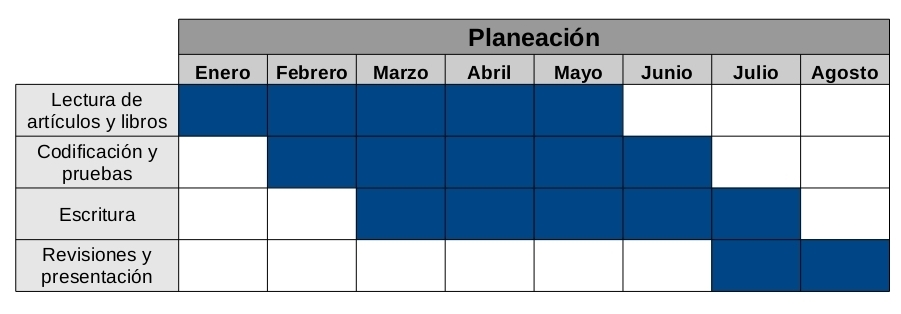
\includegraphics[width=10cm]{sss.jpg}
\end{figure}
\end{frame}






\section{ }
\begin{frame}
\begin{center}
Gracias.
\end{center}
\end{frame}




\end{document}




